\documentclass{article}
\usepackage[utf8]{inputenc}
\usepackage[absolute]{textpos}
\usepackage[default]{raleway}
\usepackage{titlesec, comment, tabularx, longtable, makecell, listings, array, setspace, geometry, graphicx, xcolor, xparse, fancyvrb, relsize, fancyhdr, booktabs, hyperref, float}
\usepackage{colortbl}
\usepackage{lipsum}
%\geometry{a4paper, left=2cm, right=2cm, top=2cm, bottom=2.5cm}
\renewcommand{\headrulewidth}{0pt}

% Definisci uno stile per i comandi git
\definecolor{light-gray}{gray}{0.92}

\lstdefinestyle{code}{
    frame=single,
    framesep=1mm,
    rulecolor=\color{light-gray},
    backgroundcolor=\color{light-gray},
    basicstyle=\ttfamily,
}

% ----------------------------- Definizione tabella ---------------------------

\newcolumntype{C}[1]{>{\centering\arraybackslash}m{#1}}

%\setcellgapes{2ex} % Imposta l'altezza dell'header (2ex)


% ------------------------------Metadati indice --------------------------------
\title{\textbf{\fontsize{28}{6}\selectfont Indice}}
\author{\fontsize{14}{6}\selectfont ByteOps}
\date{}


% -----------------------------Creazione footer --------------------------------

\pagestyle{fancy}
\fancyhf{}
\renewcommand{\footrulewidth}{0.4pt}
\lfoot{
    \parbox[c]{2cm}{
\includegraphics[width=2cm]{../Images/logo.png}}
    \textcolor[RGB]{120, 120, 120}{$\cdot$ Analisi dei requisiti}
}
\rfoot{\thepage}

% --------------------------Modifica formato hyperlinks ------------------------

\hypersetup{
    colorlinks=true,
    linkcolor=black,
    filecolor=black,      
    pdftitle={Norme di Progetto},
    pdfpagemode=FullScreen,
}

% ------------------------------- Valore sotto-paragrafi indice --------------------------------------

\setcounter{secnumdepth}{4}
\setcounter{tocdepth}{4}

\titleformat{\section}
{\normalfont\huge\bfseries}{\thesection}{0.2cm}{}
\titlespacing*{\paragraph}{0pt}{0.5cm}{0.1cm}

\titleformat{\subsection}
{\normalfont\Large\bfseries}{\thesubsection}{0.2cm}{}
\titlespacing*{\paragraph}{0pt}{0.5cm}{0.1cm}

\titleformat{\subsubsection}
{\normalfont\large\bfseries}{\thesubsubsection}{0.2cm}{}
\titlespacing*{\paragraph}{0pt}{0.5cm}{0.1cm}

\titleformat{\paragraph}
{\normalfont\normalsize\bfseries}{\theparagraph}{0.2cm}{}
\titlespacing*{\paragraph}{0pt}{0.5cm}{0.1cm}

% ------------------------------- Front Page ---------------------------------------

\begin{document}

% --------------------------Aggiunta firma finale ------------------------
%\begin{textblock*}{\textwidth}(0.85\textwidth, 1.16\textheight)
%   Il responsabile: Nome Cognome
%\end{textblock*}
% ------------------------------------------------------------------------

\pagestyle{fancy}
\begin{center}
    
\includegraphics[width = 0.7\textwidth]{../Images/logo.png} \\
    \vspace{0.2cm}
    \textcolor[RGB]{60, 60, 60}{\textit{ByteOps.swe@gmail.com}} \\
    \vspace{1cm}
    \fontsize{16}{6}\selectfont Analisi dei requisiti\\
    \vspace{0.5cm}
\end{center}

\section*{Informazioni documento}
\def\arraystretch{1.2}
\begin{tabular}{>{\raggedleft\arraybackslash}p{0.2\textwidth}|>{\raggedright\arraybackslash}p{0.6\textwidth}c}
    \hline
    \addlinespace
    \textbf{Redattori}    & A. Barutta\\ & R.Smanio \vspace{10pt} \\
    \textbf{Verificatori} & E. Hysa \vspace{10pt} \\
    \textbf{Destinatari}  & ByteOps\\ & T. Vardanega   \\ & R. Cardin \vspace{10pt} \\
\end{tabular}
\pagebreak

% ------------------------- Changelog ----------------------------

\section*{Registro delle modifiche}

\begin{tabular}{|C{1.5cm}|C{2cm}|C{2cm}|C{2cm}|C{5cm}|}
    \hline
    \textbf{Versione} & \textbf{Data} & \textbf{Autore} & \textbf{Verificatore} & \textbf{Dettaglio} \\
    \hline \hline
    \label{Git_Action_Version} 0.2.0    
             & 22/11/2023    & \makecell{A. Barutta\\ R. Smanio}    & E. Hysa          & Sez. R. Funzionali        \\
    \hline
    0.1.1             & 15/11/2023    & \makecell{A. Barutta\\ R. Smanio}    & E. Hysa          &  \makecell{Integrazione di casi d'uso}       \\
    \hline
    0.1.0             & 12/11/2023    & \makecell{A. Barutta\\ R. Smanio}    & E. Hysa          &  \makecell{Introduzione \\ D. Prodotto \\ Sez. casi d'uso}       \\
    \hline
\end{tabular}
\pagebreak

% ------------------------- Generazione automatica indice ----------------------
\setstretch{1.5}
\maketitle
\thispagestyle{fancy}
\tableofcontents
\listoffigures % Indice delle figure
\setstretch{1.2}
\pagebreak

% ------------------------ INIZIO DOCUMENTO ----------------------
\flushleft

\section{Introduzione}
\subsection{Scopo del documento}
Lo scopo del documento è di descrivere i casi d'uso e i requisiti del progetto InnovaCity,
dopo un'attenta analisi del Capitolato C6 dell'azienda SyncLab e dal
confronto con i responsabili attraverso incontri online su Google Meet.
\subsection{Glossario}
È stato adottato un Glossario per la raccolta delle principali definizioni e terminologie di termini potenzialmente ambigui presenti nella documentazione.
È possibile individuare un termine presente nel Glossario per mezzo di un G a pedice del termine.
(ex: cella\(_G\).
\section{Descrizione del prodotto}
\subsection{Obiettivi del prodotto}
Sviluppare una piattaforma di monitoraggio di una "Smart City" che consenta di avere sotto
controllo lo stato di salute della città in modo tale da prendere decisioni veloci, efficaci
ed analizzare poi gli effetti conseguenti.
A tale scopo il proponente richiede di simulare dei sensori posti in diverse aree per reperire
informazioni relative alle condizioni della città come, ad esempio, temperatura, umidità,
polveri sottili nell’aria, traffico, livelli di acqua, stato di riempimento delle isole ecologiche,
guasti elettrici e molto altro.
I dati trasmessi in tempo reale dai sensori devono poter essere memorizzati in un database
in modo tale da renderli disponibili per la visualizzazione tramite una dashboard, composta anche da widget e grafici, per una visione d’insieme delle condizioni della città in
tempo reale.
L’applicativo potrà consentire alle autorità locali di prendere decisioni informate e tempestive sulla gestione delle risorse e sull’implementazione di servizi e, inoltre, si potrebbe
rivelare uno strumento essenziale per coinvolgere i cittadini nella gestione e nel miglioramento della città.
\vspace{0.3cm}

L’implementazione di una città monitorata da sensori rappresenta un approccio promettente
nell’ottica di ottimizzare l’efficienza e la qualità della vita urbana. Tale sistema può consentire
una raccolta continua di dati e informazioni cruciali, fornendo una base solida per
l’ottimizzazione dei servizi pubblici, la gestione del traffico, la sicurezza e la sostenibilità
ambientale.


\subsection{Funzionalità del prodotto}

Il software di monitoraggio della Smart City è progettato per offrire una serie di funzionalità cruciali per gestire e migliorare le condizioni della città. Le principali funzionalità includono:

\begin{enumerate}
    \item \textbf{Simulazione di Sensori:} Il software consente la simulazione di sensori posizionati in diverse aree della città per raccogliere informazioni su parametri come temperatura, umidità, polveri sottili nell’aria, traffico, livelli di acqua, stato di riempimento delle isole ecologiche, guasti elettrici, e altro ancora.

    \item \textbf{Monitoraggio in Tempo Reale:} Il sistema raccoglie dati in tempo reale dai sensori simulati, fornendo uno stato aggiornato della città.

    \item \textbf{Memorizzazione Dei Dati:} I dati trasmessi dai sensori vengono memorizzati in un database per garantire la disponibilità a lungo termine e consentire analisi storiche.

    \item \textbf{Visualizzazione attraverso Dashboard:} Gli utenti possono accedere a una dashboard che offre una visione d’insieme delle condizioni della città in tempo reale. La dashboard è composta da widget e grafici che facilitano la comprensione e l'analisi dei dati.

    \item \textbf{Visualizzazione punteggio di salute:} Le informazioni ottenute dai simulatori consentono al sistema di calcolare un indice di benessere, valutato su una scala da zero a cento in base all'ultima rilevazione di ciascun sensore. Un punteggio più alto riflette condizioni di vita cittadine ottimali.

    \item \textbf{Supporto alle Decisioni:} L'applicativo fornisce alle autorità locali strumenti per prendere decisioni informate e tempestive sulla gestione delle risorse e sull'implementazione di servizi.

    \item \textbf{Coinvolgimento dei Cittadini:} Il software può essere utilizzato come strumento per coinvolgere i cittadini nella gestione e nel miglioramento della città, fornendo loro accesso alle informazioni e coinvolgendoli attivamente nelle decisioni.

\end{enumerate}
\subsection{Caratteristiche utente}
\textbf{Autorità Locali:} Gli utenti principali sono le autorità locali responsabili della gestione e del monitoraggio della Smart City. Questi utenti devono essere in grado di prendere decisioni informate sulla base delle informazioni raccolte e analizzate dal sistema.
\begin{itemize}
    \item L'utente dovrà utilizzare un dispositivo (Desktop o Mobile) connesso alla rete per poter accedere alla piattaforma.
\end{itemize}

\subsection{Tecnologie}
\begin{itemize}
    \item \textbf{Python} \textit{(Faker o simili)}\textbf{:} Per la simulazione delle informazioni provenienti dai sensori.
    \item \textbf{Apache Kafka:} Broker per disaccoppiare lo stream di informazioni provenienti dai simulatori dei sensori.
    \item \textbf{ClickHouse:} database \textit{OLAP} per mantenere i numerosi dati provenienti dai sensori.
    \item \textbf{Grafana:} piattaforma di Data Visualization per permettere il monitoraggio della città e la visualizzazione delle informazioni raccolte dai sensori.
\end{itemize}

\begin{figure}[H]
    \centering
    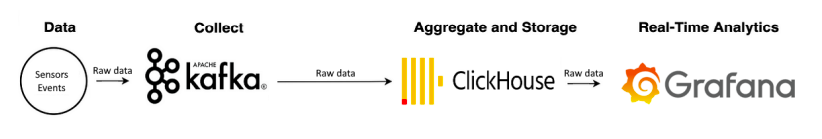
\includegraphics[width=0.9\textwidth]{Images/stackTecnologico.PNG}
    \caption{Stack tecnologico}
    \label{fig:stackTecnologico}
\end{figure}

\section{Casi d'uso}
\subsection{Introduzione}
Questa sezione illustra i casi d'uso delineati dopo l'analisi del Capitolato, il confronto con il proponente e le discussioni tra gli Analisti del gruppo. Ognuno di essi è identificato da un codice, la cui struttura è dettagliata nelle Norme di Progetto v1.0.0.
\subsection{Attori}
L'attore principale sarà unicamente l'autorità locale, il quale avrà accesso esclusivo alla visualizzazione della dashboard relativa allo stato della città, l'applicazione non richiede autenticazione.
\subsection{Elenco dei casi d'uso}


%______________________________________________________________________%

\begin{figure}[H]
    \centering
    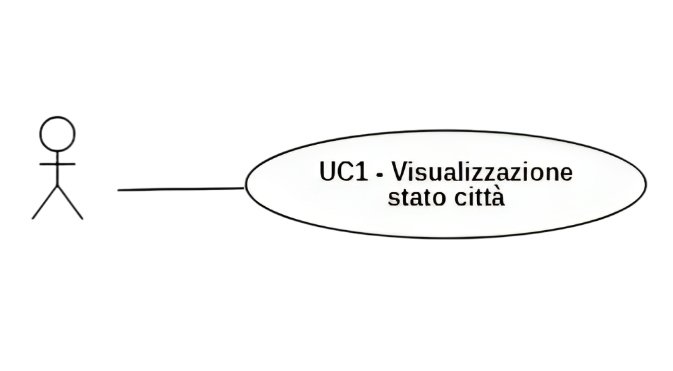
\includegraphics[width=0.9\textwidth]{Images/uc1.png}
    \caption{UC1 - Visualizzazione stato città}
    \label{fig:UC1}
\end{figure}

\subsubsection{UC1 - Visualizzazione stato città}
\begin{itemize}
    \item \textbf{Attore principale:} Autorità locale;
    \item \textbf{Descrizione:} L'autorità locale accede alla dashboard per visualizzare in tempo reale i dati provenienti dai diversi tipi di sensori, consentendo una rapida valutazione dello stato generale della città;
    \item \textbf{Scenario principale:}
          \begin{enumerate}
              \item L'utente accede alla piattaforma per la visualizzazione della dashboard ;
          \end{enumerate}
    \item \textbf{Precondizioni:}
          \begin{itemize}
              \item  Almeno un sensore è attivo e ha trasmesso dati;
          \end{itemize}
    \item \textbf{Postcondizioni:}
          \begin{itemize}
              \item      L'utente ha una visione aggiornata dello stato di salute della città tramite widget e grafici interattivi aggiornati in tempo reale, una mappa dei sensori presenti nella città e un punteggio di salute relativo alla città.
          \end{itemize}
    \item \textbf{User story associata:}
          \begin{itemize}
              \item Come Autorità Locale, voglio accedere alla dashboard per visualizzare in tempo reale i dati provenienti dai diversi tipi di sensori presenti nella città. Questo mi consentirà di valutare rapidamente lo stato generale della città e prendere decisioni informate per migliorare la situazione.
          \end{itemize}
\end{itemize}
%______________________________________________________________________%

\begin{figure}[H]
    \centering
    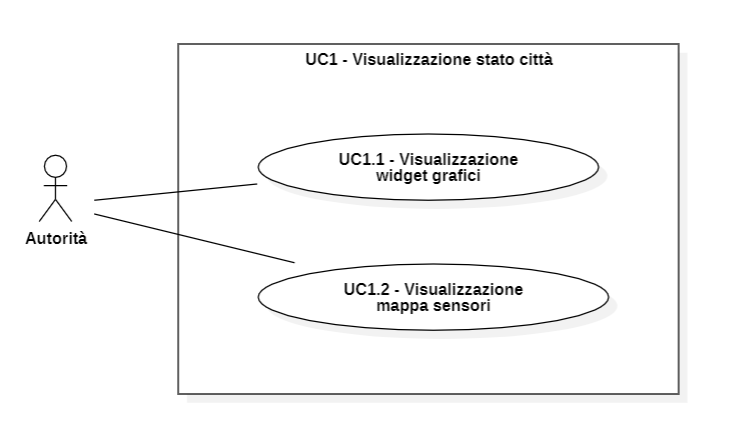
\includegraphics[width=0.9\textwidth]{Images/uc1_Subcase.PNG} 
    \caption{Sottocasi UC1 - Visualizzazione stato città}
    \label{fig:UC1_sub}
\end{figure}

\subsubsection{UC1.1 - Visualizzazione widget grafici}
\begin{itemize}
    \item \textbf{Attore principale:} Autorità locale;
    \item \textbf{Descrizione:} L'autorità locale accede alla dashboard della città e visualizza un widget contente un grafico aggiornato in tempo reale per ogni tipologia di sensore che trasmette al sistema.
    \item \textbf{Scenario principale:}
          \begin{enumerate}
              \item L'utente visualizza un widget contente un grafico per ogni tipologia di sensore che trasmette dati presente nella città.
          \end{enumerate}
    \item \textbf{Precondizioni:}
          \begin{itemize}
              \item  Almeno un sensore è attivo e ha trasmesso dati;
              \item L'utente si trova nella dashboard della città.(UC1)
          \end{itemize}
    \item \textbf{Postcondizioni:}
          \begin{itemize}
              \item      L'utente ha una visione grafica aggiornata in tempo reale sui dati registrati per ogni tipologia di sensore.
          \end{itemize}
    \item \textbf{User story associata:}
          \begin{itemize}
              \item Come un autorità locale
                    Voglio visualizzare grafici aggiornati in tempo reale per ogni tipologia di sensore nella dashboard della città.
          \end{itemize}

\end{itemize}

%______________________________________________________________________%
\subsubsection{UC1.2 - Visualizzazione mappa sensori}
\begin{itemize}
    \item \textbf{Attore principale:} Autorità locale;
    \item \textbf{Descrizione:} L'autorità locale accede alla dashboard della città e visualizza una mappa con una visione dei sensori posizionati nella città.
    \item \textbf{Scenario principale:}
          \begin{enumerate}
              \item L'utente visualizza una mappa contenente i sensori nella corretta posizione. (i sensori sono etichettati per riconoscere la tipologia)
          \end{enumerate}
    \item \textbf{Precondizioni:}
          \begin{itemize}
              \item  Almeno un sensore è attivo e ha trasmesso dati;
              \item L'utente si trova nella dashboard della città. (UC1)
          \end{itemize}
    \item \textbf{Postcondizioni:}
          \begin{itemize}
              \item      L'utente ha una visione grafica aggiornata della mappa dei sensori nella città.
          \end{itemize}
    \item \textbf{User story associata:}
          \begin{itemize}
              \item Come autorità locale, voglio essere in grado di visualizzare una mappa contenente i sensori attivi e operativi all'interno della città. La mappa deve mostrare chiaramente la posizione di ciascun sensore e deve essere etichettata per consentire un riconoscimento immediato della tipologia di ogni sensore.
          \end{itemize}
\end{itemize}

%______________________________________________________________________%

\begin{figure}[H]
    \centering
    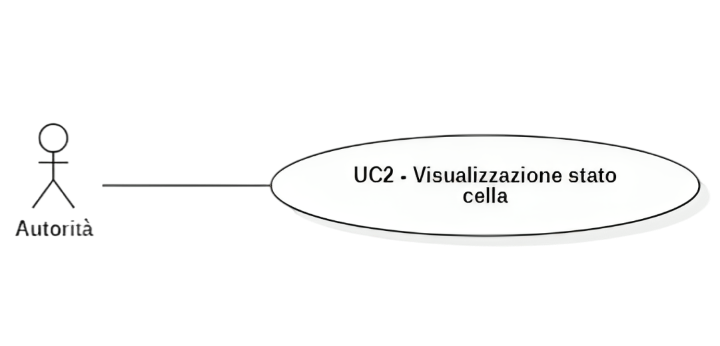
\includegraphics[width=0.9\textwidth]{Images/uc2.png}
    \caption{UC2 - Visualizzazione stato cella}
    \label{fig:UC2}
\end{figure}

\subsubsection{UC2 - Visualizzazione stato cella}
\begin{itemize}
    \item \textbf{Attore principale:} Autorità locale;
    \item \textbf{Descrizione:} L'autorità locale effettua la selezione della cella, ossia la specifica zona urbana, al fine di visualizzare in tempo reale i dati provenienti da varie tipologie di sensori ubicati nella suddetta area. Ciò permette una valutazione reapida dello stato complessivo della cella.
    \item \textbf{Scenario principale:}
          \begin{enumerate}
              \item L'utente seleziona la cella per la quale desidera visualizzare la dashboard contenente esclusivamente i dati correlati a essa.
          \end{enumerate}
    \item \textbf{Precondizioni:}
          \begin{itemize}
              \item  Almeno un sensore presente nella cella è attivo e ha trasmesso dati;
              \item L'utente di trova  nella piattaforma per la visualizzazione della dashboard sullo stato della città (UC1);
          \end{itemize}
    \item \textbf{Postcondizioni:}
          \begin{itemize}
              \item  L'utente ha una visione aggiornata dello stato di salute della cella tramite widget e grafici interattivi aggiornati in tempo reale sulla base di dati correlati esclusivamente alla cella
                    Inoltre visualizza una mappa dei sensori presenti nella cella e un punteggio di salute relativo alla cella.
          \end{itemize}
    \item \textbf{User story associata:}
          \begin{itemize}
              \item Come autorità locale, desidero poter selezionare una specifica cella urbana sulla piattaforma al fine di visualizzare immediatamente i dati provenienti da vari sensori presenti nell'area. Questo mi permetterà di valutare rapidamente lo stato complessivo della cella e prendere decisioni informate.
          \end{itemize}
\end{itemize}

%______________________________________________________________________%

\begin{figure}[H]
    \centering
    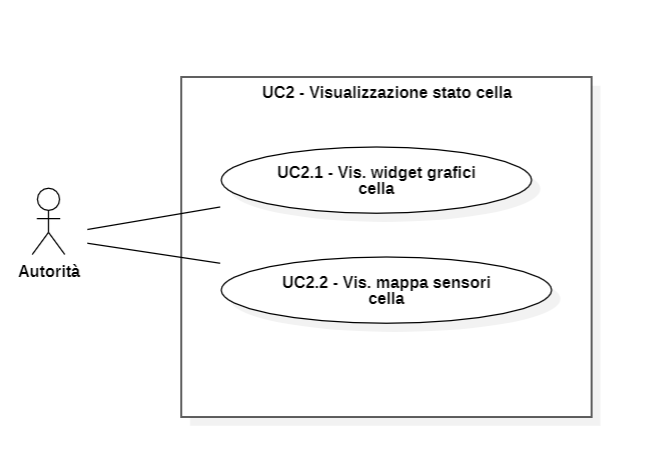
\includegraphics[width=0.9\textwidth]{Images/uc2_Subcase.PNG}
    \caption{Sottocasi UC2 - Visualizzazione stato cella}
    \label{fig:UC2_sub}
\end{figure}

\subsubsection{UC2.1 - Visualizzazione widget grafici cella}
\begin{itemize}
    \item \textbf{Attore principale:} Autorità locale;
    \item \textbf{Descrizione:} L'autorità locale accede alla dashboard della cella e visualizza un widget contente un grafico aggiornato in tempo reale per ogni tipologia di sensore che trasmette al sistema.
    \item \textbf{Scenario principale:}
          \begin{enumerate}
              \item L'utente visualizza un widget contente un grafico per ogni tipologia di sensore che trasmette dati presente nella cella.
          \end{enumerate}
    \item \textbf{Precondizioni:}
          \begin{itemize}
              \item  Almeno un sensore nella cella è attivo e ha trasmesso dati;
              \item L'utente si trova nella dashboard relativa ad una cella (UC2)
          \end{itemize}
    \item \textbf{Postcondizioni:}
          \begin{itemize}
              \item      L'utente ha una visione grafica aggiornata in tempo reale sui dati registrati per ogni tipologia di sensore.
          \end{itemize}
    \item \textbf{User story associata:}
          \begin{itemize}
              \item Come Autorità locale voglio accedere alla dashboard della cella e visualizzare un widget contenente un grafico aggiornato in tempo reale per ogni tipologia di sensore presente nella cella,
                    in modo tale che possa ottenere una visione immediata e chiara dei dati registrati dai sensori.
          \end{itemize}
\end{itemize}
%______________________________________________________________________%
\subsubsection{UC2.2 - Visualizzazione mappa sensori cella}
\begin{itemize}
    \item \textbf{Attore principale:} Autorità locale;
    \item \textbf{Descrizione:} L'autorità locale accede alla dashboard di una cella e visualizza una mappa con una visione dei sensori posizionati nella cella.
    \item \textbf{Scenario principale:}
          \begin{enumerate}
              \item L'utente visualizza una mappa contenente soli i sensori presenti nella cella. (i sensori sono etichettati per riconoscere la tipologia)
          \end{enumerate}
    \item \textbf{Precondizioni:}
          \begin{itemize}
              \item  Almeno un sensore nella cella è attivo e ha trasmesso dati;
              \item L'utente si trova nella dashboard di una cella. (UC2)
          \end{itemize}
    \item \textbf{Postcondizioni:}
          \begin{itemize}
              \item      L'utente ha una visione grafica aggiornata della mappa dei sensori nella cella.
          \end{itemize}
    \item \textbf{User story associata:}
          \begin{itemize}
              \item Come autorità locale, voglio essere in grado di visualizzare una mappa contenente solo i sensori attivi e operativi all'interno di una specifica cella. La mappa deve mostrare chiaramente la posizione di ciascun sensore e deve essere etichettata per consentire un riconoscimento immediato della tipologia di ogni sensore.
          \end{itemize}
\end{itemize}

%______________________________________________________________________%

\begin{figure}[H]
    \centering
    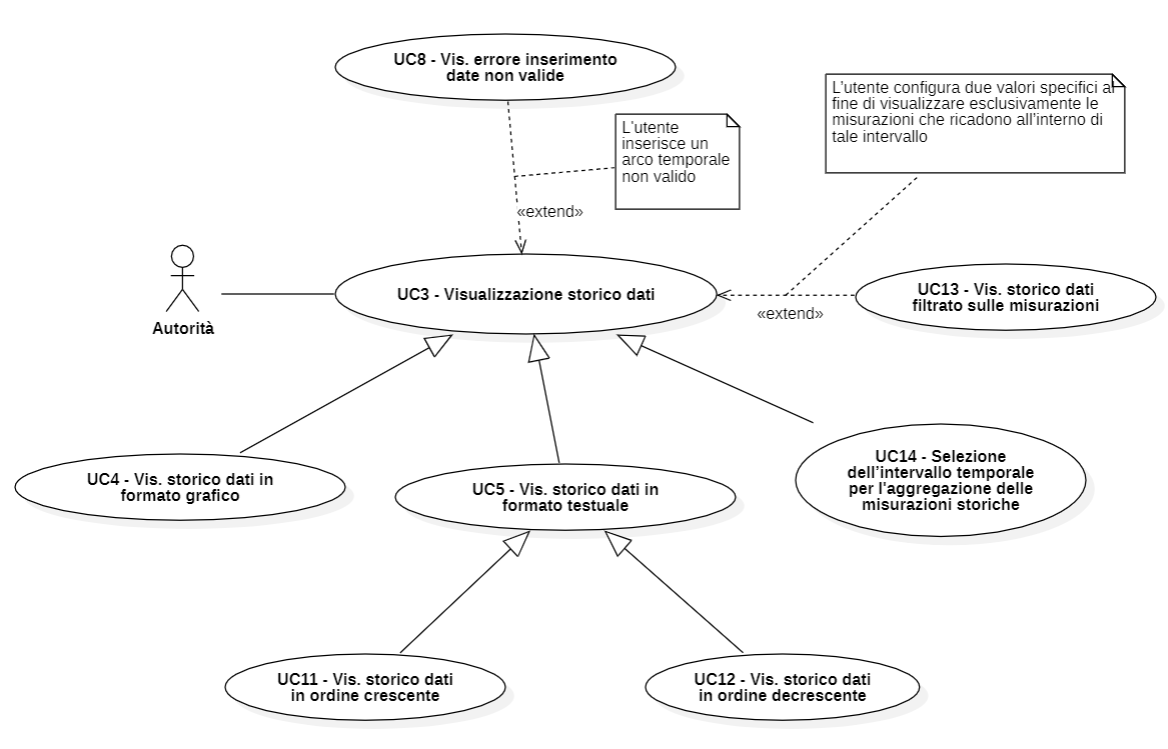
\includegraphics[width=0.9\textwidth]{Images/uc3.png}
    \caption{UC3 - Visualizzazione storico dati }
    \label{fig:UC3}
\end{figure}
\subsubsection{UC3 - Visualizzazione storico dati }

\begin{itemize}
    \item \textbf{Attore principale:} Autorità locale;
    \item \textbf{Descrizione:} L'autorità locale procede all'accesso alla piattaforma e visualizza dati storici dei sensori.
    \item \textbf{Scenario principale:}
          \begin{enumerate}
              \item L'utente seleziona la visulizzazione dello storico dati dei sensori.
              \item L'utente seleziona l'arco temporale di visualizzazione dello storico, (Di default tutti i dati)
          \end{enumerate}
    \item \textbf{Estensioni:}
          \begin{enumerate}
              \item L'utente un arco temporale non valido (UC8).
              \item Visualizzazione storico dati filtrato sulle misurazioni (UC13)
          \end{enumerate}
    \item \textbf{Precondizioni:}
          \begin{itemize}
              \item  I/Il sensori/e di cui si vuole visualizzare i dati storici ha trasmesso dati.
              \item  L'utente visualizza una dashboard (UC1) (UC2);
          \end{itemize}
    \item \textbf{Postcondizioni:}
          \begin{itemize}
              \item  L'utente ha una visione esclusiva dello storico dei dati trasmessi  dai/l sensori/e.
          \end{itemize}
    \item \textbf{User story associata:}
          \begin{itemize}
              \item Come autorità locale,
                    Voglio accedere alla piattaforma e visualizzare i dati storici dei sensori tra due date (Di default, la
                    visualizzazione deve includere
                    tutti i dati disponibili),
                    in modo da analizzare le tendenze nel tempo per prendere decisioni informate sulla gestione urbana.
          \end{itemize}
\end{itemize}

\subsubsection{UC4 - Visualizzazione storico dati in formato testuale}
\begin{itemize}
    \item \textbf{Attore principale:} Autorità locale;
    \item \textbf{Descrizione:} L’autorità locale seleziona i/il sensore/i della quale vuole visionare lo storico dei dati e imposta la visulizzazione in formato testuale: (TIMESTAMP, Dato)
    \item \textbf{Scenario principale:}
          \begin{enumerate}
              \item L'utente imposta la visualizzazione in formato testuale.
          \end{enumerate}
    \item \textbf{Precondizioni:}
          \begin{itemize}
              \item  I/Il sensori/e di cui si vuole visualizzare i dati storici ha trasmesso dati.
              \item  L'utente si trova in un interfaccia per la visualizzazione di uno storico dati (UC3)
          \end{itemize}
    \item \textbf{Postcondizioni:}
          \begin{itemize}
              \item  L'utente ha una visione dello storico dei dati trasmessi nel formato (TIMESTAMP, dato)
          \end{itemize}
    \item \textbf{User story associata:}
          \begin{itemize}
              \item Come autorità locale,
                    desidero visualizzare lo storico dei dati in formato testuale (TIMESTAMP, Dato),
                    In modo da avere una visione dettagliata delle informazioni trasmesse dai sensori.
          \end{itemize}
\end{itemize}
\subsubsection{UC11 - Visualizzazione storico dati in ordine crescente}
\begin{itemize}
    \item \textbf{Attore principale:} Autorità locale;
    \item \textbf{Descrizione:} L’autorità locale seleziona i/il sensore/i della quale vuole visionare lo storico dei dati in formato testuale in ordine crescente rispetto alle misurazioni del/i sensore/i.
    \item \textbf{Scenario principale:}
          \begin{enumerate}
              \item L'utente imposta la visualizzazione in ordine crescente.
          \end{enumerate}
    \item \textbf{Precondizioni:}
          \begin{itemize}
              \item  I/Il sensori/e di cui si vuole visualizzare i dati storici ha trasmesso dati.
              \item  L'utente si trova in un interfaccia per la visualizzazione di uno storico dati in formato testuale (UC4)
          \end{itemize}
    \item \textbf{Postcondizioni:}
          \begin{itemize}
              \item  L'utente ha una visione dello storico dei dati trasmessi nel formato (TIMESTAMP, dato) in ordine crescente rispetto alle misurazioni.
          \end{itemize}
    \item \textbf{User story associata:}
          \begin{itemize}
              \item Come autorità locale, desidero essere in grado di visualizzare lo storico dei dati provenienti dai sensori in formato testuale, ordinati in modo crescente rispetto alla misurazione del/i sensore/i, al fine di identificare facilmente tendenze, cambiamenti o pattern nel tempo.
          \end{itemize}
\end{itemize}
\subsubsection{UC12 - Visualizzazione storico dati in ordine decrescente}
\begin{itemize}
    \item \textbf{Attore principale:} Autorità locale;
    \item \textbf{Descrizione:} L’autorità locale seleziona i/il sensore/i della quale vuole visionare lo storico dei dati in formato testuale in ordine decrescente rispetto alle misurazioni del/i sensore/i.
    \item \textbf{Scenario principale:}
          \begin{enumerate}
              \item L'utente imposta la visualizzazione in ordine decrescente.
          \end{enumerate}
    \item \textbf{Precondizioni:}
          \begin{itemize}
              \item  I/Il sensori/e di cui si vuole visualizzare i dati storici ha trasmesso dati.
              \item  L'utente si trova in un interfaccia per la visualizzazione di uno storico dati in formato testuale (UC4)
          \end{itemize}
    \item \textbf{Postcondizioni:}
          \begin{itemize}
              \item  L'utente ha una visione dello storico dei dati trasmessi nel formato (TIMESTAMP, dato) in ordine decrescente rispetto alle misurazioni.
          \end{itemize}
    \item \textbf{User story associata:}
          \begin{itemize}
            \item Come autorità locale, desidero essere in grado di visualizzare lo storico dei dati provenienti dai sensori in formato testuale, ordinati in modo decrescente rispetto alla misurazione del/i sensore/i, al fine di identificare facilmente tendenze, cambiamenti o pattern nel tempo.
          \end{itemize}
\end{itemize}

\subsubsection{UC5 - Visualizzazione storico dati in formato grafico}
\begin{itemize}
    \item \textbf{Attore principale:} Autorità locale;
    \item \textbf{Descrizione:} L’autorità locale seleziona i/il sensore/i della quale vuole visionare lo storico dei dati e imposta la visulizzazione in formato grafico.
    \item \textbf{Scenario principale:}
          \begin{enumerate}
              \item L'utente imposta la visualizzazione in formato grafico.
          \end{enumerate}
    \item \textbf{Precondizioni:}
          \begin{itemize}
              \item  I/Il sensori/e di cui si vuole visualizzare i dati storici ha trasmesso dati.
              \item  L'utente si trova in un interfaccia per la visualizzazione di uno storico dati (UC3).
          \end{itemize}
    \item \textbf{Postcondizioni:}
          \begin{itemize}
              \item  L'utente ha una visione dello storico dei dati trasmessi nel formato grafico.
          \end{itemize}
    \item \textbf{User story associata:}
          \begin{itemize}
              \item Come Autorità locale, voglio visualizzare lo storico dei dati in formato grafico per analizzarne le tendenze nel tempo.
          \end{itemize}
\end{itemize}

\subsubsection{UC14 -  Selezione dell'intervallo temporale per l'aggregazione delle misurazioni storiche}
\begin{itemize}
    \item \textbf{Attore principale:} Autorità locale;
    \item \textbf{Descrizione:} L'autorità locale ha la capacità di selezionare l'intervallo temporale desiderato per l'aggregazione delle misurazioni nel contesto di un'unica visualizzazione dati. Tale intervallo può essere specificato in termini di secondo, minuto, ora, giorno, mese o anno, al fine di personalizzare la scala temporale dell'analisi.
    \item \textbf{Scenario principale:}
          \begin{enumerate}
             \item L'utente sceglie tra le opzioni di aggregazione un intervallo temporale disponibili tra secondo, minuto, ora, giorno, mese o anno.
             \item Il sistema adatta dinamicamente la rappresentazione dei dati, inclusi i grafici, secondo l'intervallo temporale di aggregazione selezionato.
          \end{enumerate}
    \item \textbf{Precondizioni:}
          \begin{itemize}
              \item  L'utente si trova in un interfaccia per la visualizzazione di uno storico dati.  (UC3)
          \end{itemize}
    \item \textbf{Postcondizioni:}
          \begin{itemize}
              \item  L'utente ottiene una visualizzazione chiara e personalizzata delle misurazioni aggregate sull'intervallo temporale d'appartenenza specificato.
          \end{itemize}
    \item \textbf{User story associata:}
          \begin{itemize}
              \item Come autorità locale, desidero essere in grado di personalizzare l'intervallo temporale di aggregazione delle misurazioni, scegliendo tra le opzioni di secondo, minuto, ora, giorno, mese o anno. Questa funzionalità mi consentirà di adattare la visualizzazione dei dati alle mie specifiche esigenze temporali, agevolando l'analisi dettagliata dei trend e delle variazioni nel corso del tempo.
          \end{itemize}
\end{itemize}

\subsubsection{UC8 - Inserimento date non valide}
\begin{itemize}
    \item \textbf{Attore principale:} Autorità locale;
    \item \textbf{Descrizione:} L’autorità locale seleziona date di arco temporale non valide. (Data fine precedente a data inizio, Arco temporale precedente o antecedente all'inizio della trasmissione dati)
    \item \textbf{Scenario principale:}
          \begin{enumerate}
              \item L'utente imposta due date delimitanti entro cui intende esaminare l'andamento storico delle informazioni.
              \item Le date inserite non sono valide.
          \end{enumerate}
    \item \textbf{Precondizioni:}
          \begin{itemize}
              \item  L'utente si trova in un interfaccia per la visualizzazione di uno storico dati.  (UC3)
              \item L'utente imposta due date delimitanti entro cui intende esaminare l'andamento storico delle informazioni
                    non valide.
          \end{itemize}
    \item \textbf{Postcondizioni:}
          \begin{itemize}
              \item  L'utente riceve una notifica di errore che richiede il reinserimento di date valide.
          \end{itemize}
    \item \textbf{User story associata:}
          \begin{itemize}
              \item Come autorità locale, voglio essere avvisato quando inserisco date non valide durante la configurazione dello storico dati, in modo da correggere immediatamente e ottenere informazioni accurate.
          \end{itemize}
\end{itemize}
\subsubsection{UC13 - Visualizzazione storico dati filtrato sulle misurazioni}
\begin{itemize}
    \item \textbf{Attore principale:} Autorità locale;
    \item \textbf{Descrizione:} L’autorità locale seleziona i/il sensore/i della quale vuole visionare lo storico dei dati e filtra la visualizzazione ai soli dati compresi tra due valori.
    \item \textbf{Scenario principale:}
          \begin{enumerate}
              \item L'utente configura due valori specifici al fine di visualizzare esclusivamente le misurazioni che ricadono all'interno di tale intervallo.
          \end{enumerate}
    \item \textbf{Precondizioni:}
          \begin{itemize}
              \item  I/Il sensori/e di cui si vuole visualizzare i dati storici ha trasmesso dati.
              \item  L'utente si trova in un interfaccia per la visualizzazione di uno storico dati (UC3)
          \end{itemize}
    \item \textbf{Postcondizioni:}
          \begin{itemize}
              \item  L'utente accede a una rappresentazione dello storico dei dati trasmessi, la cui visualizzazione è stata filtrata esclusivamente per includere le misurazioni con il dato compreso tra i due valori specificati.
          \end{itemize}
    \item \textbf{User story associata:}
          \begin{itemize}
            \item In qualità di utente, desidero avere la possibilità di filtrare la visualizzazione dello storico dei dati in base alle misurazioni del sensore comprese tra due valori specifici. Questo mi consentirà di analizzare in modo più mirato e focalizzato i dati che rientrano in un determinato intervallo, facilitando l'identificazione di pattern o anomalie significative.
          \end{itemize}
\end{itemize}


%______________________________________________________________________%

\begin{figure}[H]
    \centering
    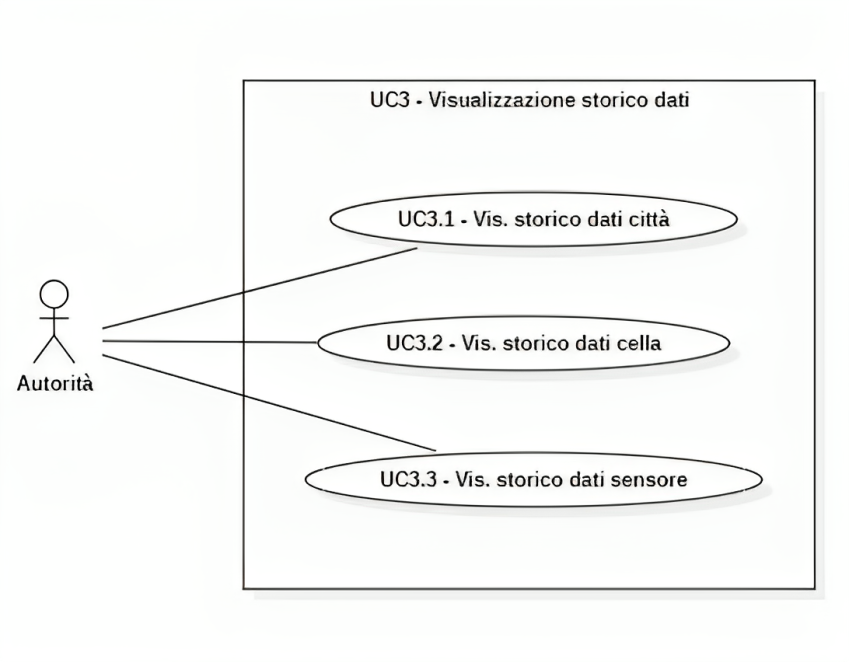
\includegraphics[width=0.9\textwidth]{Images/uc3_Subcase.png}
    \caption{Sottocasi UC3 - Visualizzazione storico dati }
    \label{fig:UC3_sub}
\end{figure}

\subsubsection{UC3.1 - Visualizzazione storico dati città per una specifica tipologia di sensore}
\begin{itemize}
    \item \textbf{Attore principale:} Autorità locale;
    \item \textbf{Descrizione:} L'autorità locale procede all'accesso alla piattaforma e, mediante la dashboard relativa allo stato di salute della città, effettua la selezione di una specifica categoria di sensori al fine di visualizzare esclusivamente i dati storici ad essi pertinenti.
    \item \textbf{Scenario principale:}
          \begin{enumerate}
              \item L'utente seleziona la tipologia di sensori di cui vuole visionare lo storico dei dati trasmessi.
          \end{enumerate}
    \item \textbf{Precondizioni:}
          \begin{itemize}
              \item  L'utente di trova  nella piattaforma per la visualizzazione della dashboard sullo stato della città (UC1);
              \item  Almeno un sensore della tipologia selezionata ha trasmesso dati.
          \end{itemize}
    \item \textbf{Postcondizioni:}
          \begin{itemize}
              \item  L'utente ha una visione esclusiva dello storico dei dati trasmessi da tutti sensori della tipologia selezionata.
          \end{itemize}
    \item \textbf{User story associata:}
          \begin{itemize}
              \item In quanto Autorità Locale, desidero accedere alla piattaforma e visualizzare esclusivamente lo storico dei dati trasmessi da una specifica tipologia di sensori nella città, attraverso la dashboard relativa allo stato di salute della città.
          \end{itemize}
\end{itemize}
\subsubsection{UC3.2 - Visualizzazione Storico Dati cella per una Specifica Tipologia di Sensore}
\begin{itemize}
    \item \textbf{Attore principale:} Autorità locale;
    \item \textbf{Descrizione:} L’autorità locale procede all’accesso alla piattaforma e, mediante la
          dashboard relativa allo stato di salute della cella, effettua la selezione di una specifica
          categoria di sensori al fine di visualizzare esclusivamente i dati storici ad essi pertinenti.
    \item \textbf{Scenario principale:}
          \begin{enumerate}
              \item L'utente seleziona la tipologia di sensori di cui vuole visionare lo storico dei dati trasmessi nella cella.
          \end{enumerate}
    \item \textbf{Precondizioni:}
          \begin{itemize}
              \item L'utente di trova nella piattaforma per la visualizzazione della dashboard sullo stato della cella (UC2);
              \item  Almeno un sensore della tipologia selezionata è presente nella cella ha trasmesso dati.
          \end{itemize}
    \item \textbf{Postcondizioni:}
          \begin{itemize}
              \item  L'utente ha una visione dello storico dei dati trasmessi dai sensori della tipologia selezionata presenti nella cella.
          \end{itemize}
    \item \textbf{User story associata:}
          \begin{itemize}
              \item Come autorità locale,
                    Desidero accedere alla piattaforma e visualizzare lo storico dei dati trasmessi da una specifica tipologia di sensori in una cella,
                    In modo che possa analizzare e comprendere l'andamento storico dei dati relativi a quella categoria di sensori per prendere decisioni informate sullo stato della cella.
          \end{itemize}
\end{itemize}

\subsubsection{UC3.3 - Visualizzazione Storico Dati sensore}
\begin{itemize}
    \item \textbf{Attore principale:} Autorità locale;
    \item \textbf{Descrizione:} L’autorità locale seleziona dalla mappa un sensore di cui vuole visionare lo storico dei dati trasmessi.
    \item \textbf{Scenario principale:}
          \begin{enumerate}
              \item L'utente seleziona il sensore di cui vuole visionare lo storico.
          \end{enumerate}
    \item \textbf{Precondizioni:}
          \begin{itemize}
              \item  L'utente di trova  nella piattaforma per la visualizzazione della dashboard sullo stato della città (UC1);
              \item Il sensore selezionato ha trasmesso dati.
          \end{itemize}
    \item \textbf{Postcondizioni:}
          \begin{itemize}
              \item  L'utente ha una visione dello storico dei dati trasmessi dal sensore selezionato.
          \end{itemize}
    \item \textbf{User story associata:}
          \begin{itemize}
              \item Come Autorità locale, desidero poter visualizzare lo storico dei dati trasmessi da un sensore specifico. Questo mi permetterà di analizzare e comprendere l'andamento delle misurazioni nel tempo.
          \end{itemize}
\end{itemize}

%______________________________________________________________________%

\begin{figure}[H]
    \centering
    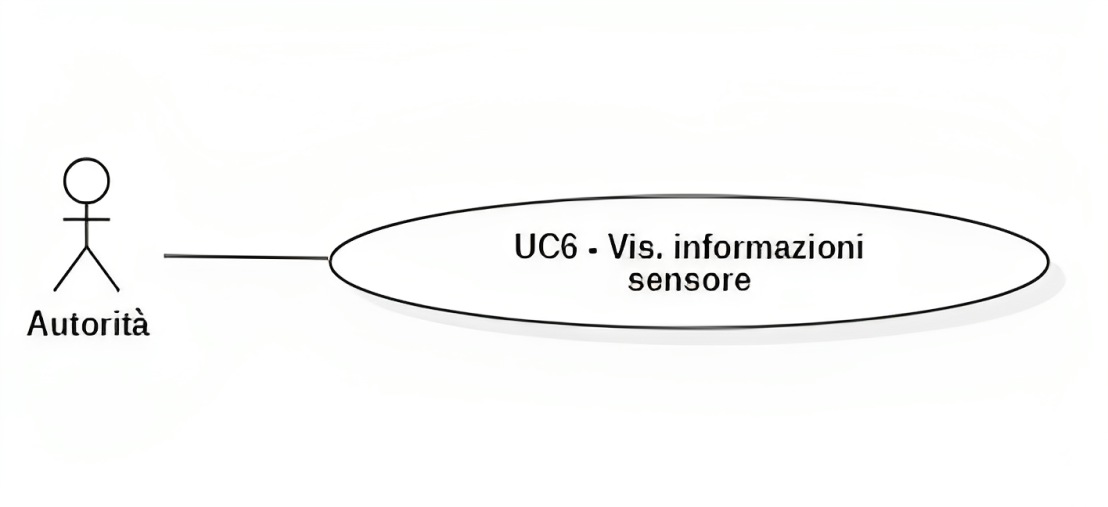
\includegraphics[width=0.9\textwidth]{Images/uc6.png}
    \caption{UC6 - Visualizzazione informazioni sensore}
    \label{fig:UC6}
\end{figure}

\subsubsection{UC6 - Visualizzazione informazioni sensore}
\begin{itemize}
    \item \textbf{Attore principale:} Autorità locale;
    \item \textbf{Descrizione:} L’autorità locale dalla pagina adibita alla visione dello storico dati di un sensore seleziona la visualizzazione delle informazioni sul sensore.
    \item \textbf{Scenario principale:}
          \begin{enumerate}
              \item L'utente seleziona la visualizzazione dell'informazioni del sensore.
          \end{enumerate}
    \item \textbf{Precondizioni:}
          \begin{itemize}
              \item  L'utente di trova nella pagina di visualizzazione dello storico dei dati di un sensore.
          \end{itemize}
    \item \textbf{Postcondizioni:}
          \begin{itemize}
              \item  L'utente ha una visione delle informazioni del sensore.
          \end{itemize}
    \item \textbf{User story associata:}
          \begin{itemize}
              \item Come Autorità locale, desidero visualizzare le informazioni dettagliate di un sensore dalla pagina dedicata al relativo storico dei dati, al fine di ottenere una visione completa delle caratteristiche e delle specifiche del sensore selezionato.
          \end{itemize}
\end{itemize}

%______________________________________________________________________%

\begin{figure}[H]
    \centering
    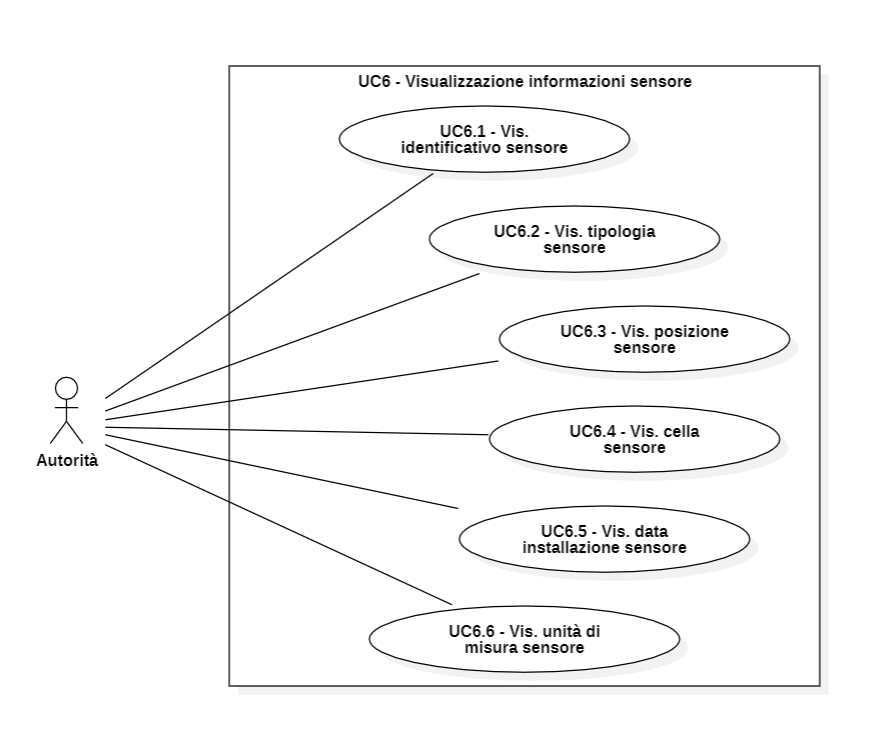
\includegraphics[width=0.9\textwidth]{Images/uc6_Subcase.PNG}
    \caption{Sottocasi UC6 - Visualizzazione informazioni sensore}
    \label{fig:UC6_sub}
\end{figure}

\subsubsection{UC6.1 - Visualizzazione Identificativo sensore}
\begin{itemize}
    \item \textbf{Attore principale:} Autorità locale;
    \item \textbf{Descrizione:} L’autorità locale dalla pagina adibita alla visione delle informazioni di un sensore visualizza il suo Identificativo.
    \item \textbf{Scenario principale:}
          \begin{enumerate}
              \item L'utente visualizza l'Identificativo del sensore.
          \end{enumerate}
    \item \textbf{Precondizioni:}
          \begin{itemize}
              \item  L'utente di trova nella pagina di visualizzazione delle informazioni di un sensore (UC6.1)
          \end{itemize}
    \item \textbf{Postcondizioni:}
          \begin{itemize}
              \item  L'utente visualizza l'Identificativo del sensore.
          \end{itemize}\item \textbf{User story associata:}
          \begin{itemize}
              \item Come Autorità Locale, desidero visualizzare l'identificativo di un sensore dalla pagina dedicata alle informazioni del sensore.
          \end{itemize}
\end{itemize}
%______________________________________________________________________%
\subsubsection{UC6.2 - Visualizzazione tipologia sensore}
\begin{itemize}
    \item \textbf{Attore principale:} Autorità locale;
    \item \textbf{Descrizione:} L’autorità locale dalla pagina adibita alla visione delle informazioni di un sensore visualizza la sua tipologia (ex. Termometro).
    \item \textbf{Scenario principale:}
          \begin{enumerate}
              \item L'utente visualizza la tipolgia del sensore.
          \end{enumerate}
    \item \textbf{Precondizioni:}
          \begin{itemize}
              \item  L'utente di trova nella pagina di visualizzazione delle informazioni di un sensore (UC6.1)
          \end{itemize}
    \item \textbf{Postcondizioni:}
          \begin{itemize}
              \item  L'utente visualizza la tipologia del sensore.
          \end{itemize}\item \textbf{User story associata:}
          \begin{itemize}
              \item Come Autorità Locale, desidero visualizzare la tipolgia di un sensore dalla pagina dedicata alle informazioni del sensore.
          \end{itemize}


\end{itemize}
%______________________________________________________________________%
\subsubsection{UC6.3 - Visualizzazione posizione sensore}
\begin{itemize}
    \item \textbf{Attore principale:} Autorità locale;
    \item \textbf{Descrizione:} L’autorità locale dalla pagina adibita alla visione delle informazioni di un sensore visualizza la sua posizione in coordinate.
    \item \textbf{Scenario principale:}
          \begin{enumerate}
              \item L'utente visualizza le coordinate del sensore.
          \end{enumerate}
    \item \textbf{Precondizioni:}
          \begin{itemize}
              \item  L'utente di trova nella pagina di visualizzazione delle informazioni di un sensore (UC6.1)
          \end{itemize}
    \item \textbf{Postcondizioni:}
          \begin{itemize}
              \item  L'utente visualizza le coordinate del sensore.
          \end{itemize}
    \item \textbf{User story associata:}
          \begin{itemize}
              \item Come Autorità Locale, desidero visualizzare la posizione di un sensore, in coordinate, dalla pagina dedicata alle informazioni del sensore.
          \end{itemize}
\end{itemize}
%______________________________________________________________________%
\subsubsection{UC6.4 - Visualizzazione cella sensore}
\begin{itemize}
    \item \textbf{Attore principale:} Autorità locale;
    \item \textbf{Descrizione:} L’autorità locale dalla pagina adibita alla visione delle informazioni di un sensore visualizza la cella dove è installato il sensore.
    \item \textbf{Scenario principale:}
          \begin{enumerate}
              \item L'utente visualizza la cella dove è installato il sensore
          \end{enumerate}
    \item \textbf{Precondizioni:}
          \begin{itemize}
              \item  L'utente di trova nella pagina di visualizzazione delle informazioni di un sensore (UC6.1)
          \end{itemize}
    \item \textbf{Postcondizioni:}
          \begin{itemize}
              \item  L'utente visualizza la cella dove è installato il sensore
          \end{itemize}
    \item \textbf{User story associata:}
          \begin{itemize}
              \item Come Autorità Locale, desidero visualizzare la cella di appartenenza di un sensore dalla pagina dedicata alle informazioni del sensore.
          \end{itemize}
\end{itemize}
%______________________________________________________________________%
\subsubsection{UC6.5 - Visualizzazione data installazione sensore}
\begin{itemize}
    \item \textbf{Attore principale:} Autorità locale;
    \item \textbf{Descrizione:} L’autorità locale dalla pagina adibita alla visione delle informazioni di un sensore visualizza la data di installazione del sensore.
    \item \textbf{Scenario principale:}
          \begin{enumerate}
              \item L'utente visualizza la data di installazione del sensore.
          \end{enumerate}
    \item \textbf{Precondizioni:}
          \begin{itemize}
              \item  L'utente di trova nella pagina di visualizzazione delle informazioni di un sensore (UC6.1)
          \end{itemize}
    \item \textbf{Postcondizioni:}
          \begin{itemize}
              \item  L'utente visualizza la data di installazione del sensore.
          \end{itemize}
    \item \textbf{User story associata:}
          \begin{itemize}
              \item Come Autorità Locale, desidero visualizzare la data di installazione di un sensore dalla pagina dedicata alle informazioni del sensore.
          \end{itemize}
\end{itemize}
%______________________________________________________________________%
\subsubsection{UC6.6 - Visualizzazione unità misura sensore}
\begin{itemize}
    \item \textbf{Attore principale:} Autorità locale;
    \item \textbf{Descrizione:} L’autorità locale dalla pagina adibita alla visione delle informazioni di un sensore visualizza l'unità di misura del sensore.
    \item \textbf{Scenario principale:}
          \begin{enumerate}
              \item L'utente visualizza l'unità di misura del sensore.
          \end{enumerate}
    \item \textbf{Precondizioni:}
          \begin{itemize}
              \item  L'utente di trova nella pagina di visualizzazione delle informazioni di un sensore (UC6.1)
          \end{itemize}
    \item \textbf{Postcondizioni:}
          \begin{itemize}
              \item  L'utente visualizza l'unità di misura del sensore.
          \end{itemize}
    \item \textbf{User story associata:}
          \begin{itemize}
              \item Come Autorità Locale, desidero visualizzare l'unità di misura di un sensore dalla pagina dedicata alle informazioni del sensore.
          \end{itemize}
\end{itemize}
%______________________________________________________________________%

\begin{figure}[H]
    \centering
    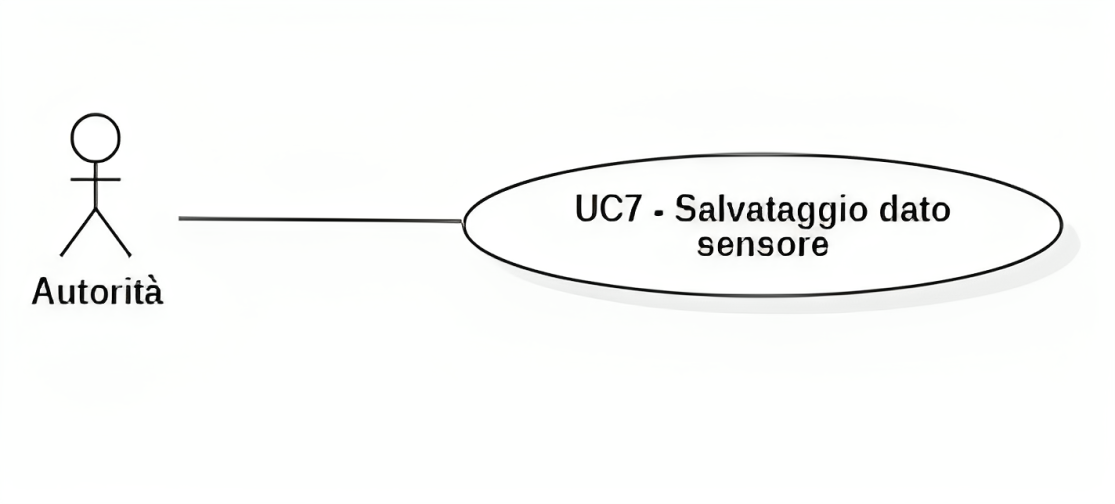
\includegraphics[width=0.9\textwidth]{Images/uc7.png}
    \caption{UC7 - Salvataggio dato sensore}
    \label{fig:UC7}
\end{figure}

\subsubsection{UC7 - Salvataggio dato storico}
\begin{itemize}
    \item \textbf{Attore principale:} Autorità locale;
    \item \textbf{Descrizione:} L’autorità locale dalle pagina adibite alla visione dello storico seleziona il salvataggio di un dato emesso tra i preferiti.
    \item \textbf{Scenario principale:}
          \begin{enumerate}
              \item L'utente salva tra i preferiti uno dei dati storici emesso.
          \end{enumerate}
    \item \textbf{Precondizioni:}
          \begin{itemize}
              \item  L'utente si trova in una pagina di visulizzazione storico dati (UC3)
              \item  Il dato che intende salvare tra i preferiti non lo era già in precedenza.
          \end{itemize}
    \item \textbf{Postcondizioni:}
          \begin{itemize}
              \item  Il dato storico viene memorizzato nella lista dei preferiti.
          \end{itemize}
    \item \textbf{User story associata:}
          \begin{itemize}
              \item n quanto autorità locale, desidero poter salvare un dato storico tra i preferiti dalla pagina dedicata alla visualizzazione degli storici, al fine di accedere rapidamente a informazioni importanti.
          \end{itemize}
\end{itemize}
%______________________________________________________________________%

\begin{figure}[H]
    \centering
    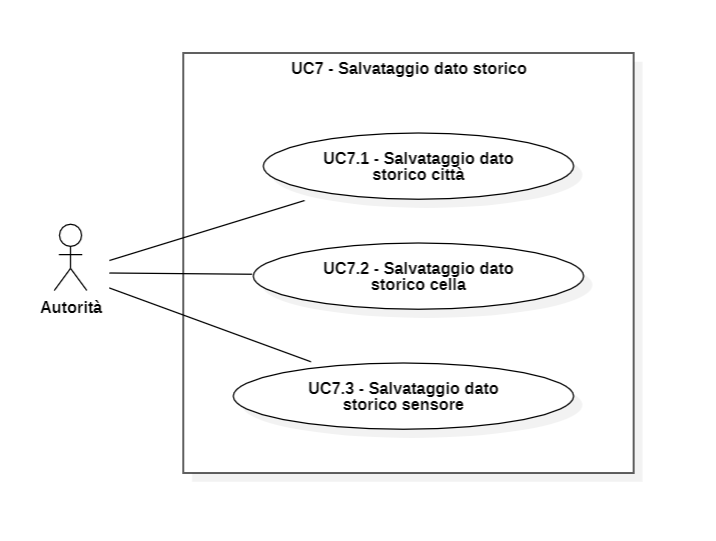
\includegraphics[width=0.9\textwidth]{Images/uc7_Subcase.PNG}
    \caption{Sottocasi UC7 - Salvataggio dato sensore}
    \label{fig:UC7_sub}
\end{figure}

\subsubsection{UC7.1 - Salvataggio dato storico citta}
\begin{itemize}
    \item \textbf{Attore principale:} Autorità locale;
    \item \textbf{Descrizione:} L’autorità locale dalla pagina adibita alla visulizzazione dello storico dati in formato testuale salva un dato emesso tra i preferiti.
    \item \textbf{Scenario principale:}
          \begin{enumerate}
              \item L'utente salva tra i preferiti uno dei dati storici della città emesso .
          \end{enumerate}
    \item \textbf{Precondizioni:}
          \begin{itemize}
              \item  L'utente si trova nella pagina di visulizzazione in formato testuale dei dati storici emessi nella città per una tipologia di sensore (UC3.3)
              \item  Il dato che intende salvare tra i preferiti non lo era già in precedenza.
          \end{itemize}
    \item \textbf{Postcondizioni:}
          \begin{itemize}
              \item  Il dato storico della città viene memorizzato nella lista dei preferiti nel
                    formato testuale: (TipoSensore,
                    TIMESTAMP, Dato).
          \end{itemize}
    \item \textbf{User story associata:}
          \begin{itemize}
              \item Come Autorità locale
                    Voglio poter salvare uno dei dati storici emessi dalla città tra i preferiti
                    In modo che possa accedere rapidamente ai dati rilevanti in futuro.
          \end{itemize}
\end{itemize}

%______________________________________________________________________%
\subsubsection{UC7.2 - Salvataggio dato storico cella}
\begin{itemize}
    \item \textbf{Attore principale:} Autorità locale;
    \item \textbf{Descrizione:} L’autorità locale dalla pagina adibita alla visulizzazione dello storico dati in formato testuale relativo ad una cella salva un dato emesso tra i preferiti.
    \item \textbf{Scenario principale:}
          \begin{enumerate}
              \item L'utente salva tra i preferiti uno dei dati storici della cella emesso .
          \end{enumerate}
    \item \textbf{Precondizioni:}
          \begin{itemize}
              \item  L'utente si trova nella pagina di visulizzazione in formato testuale dei dati storici emessi in una cella per una tipologia di sensore (UC3.2)
              \item  Il dato che intende salvare tra i preferiti non lo era già in precedenza.
          \end{itemize}
    \item \textbf{Postcondizioni:}
          \begin{itemize}
              \item  Il dato storico della città viene memorizzato nella lista dei preferiti formato testuale (Cella,
                    TipoSensore, TIMESTAMP,
                    Dato)
          \end{itemize}
    \item \textbf{User story associata:}
          \begin{itemize}
              \item Come Autorità locale
                    Voglio poter salvare uno dei dati storici emessi da una cella tra i preferiti
                    In modo che possa accedere rapidamente ai dati rilevanti in futuro.
          \end{itemize}
\end{itemize}

%______________________________________________________________________%
\subsubsection{UC7.3 - Salvataggio dato storico sensore}
\begin{itemize}
    \item \textbf{Attore principale:} Autorità locale;
    \item \textbf{Descrizione:} L’autorità locale dalla pagina adibita alla visulizzazione dei dati emessi da un sensore salva il dato tra i preferiti.
    \item \textbf{Scenario principale:}
          \begin{enumerate}
              \item L'utente salva tra i preferiti uno dei dati storici emessi dal sensore.
          \end{enumerate}
    \item \textbf{Precondizioni:}
          \begin{itemize}
              \item  L'utente si trova nella pagina di visulizzazione in formato testuale dei dati storici emessi da un sensore (UC3.3)
              \item  Il dato che intende salvare tra i preferiti non lo era già in precedenza.
          \end{itemize}
    \item \textbf{Postcondizioni:}
          \begin{itemize}
              \item  Il dato storico emesso dal sensore viene memorizzato nella lista dei preferiti nel formato testuale: (IDSensore,Cella, TipoSensore,
                    TIMESTAMP, Dato).
          \end{itemize}
    \item \textbf{User story associata:}
          \begin{itemize}
              \item Come Autorità locale voglio poter salvare uno dei dati storici emessi da un sensore tra i preferiti in modo che possa accedere rapidamente ai dati rilevanti in futuro.
          \end{itemize}
\end{itemize}

%______________________________________________________________________%

\begin{figure}[H]
    \centering
    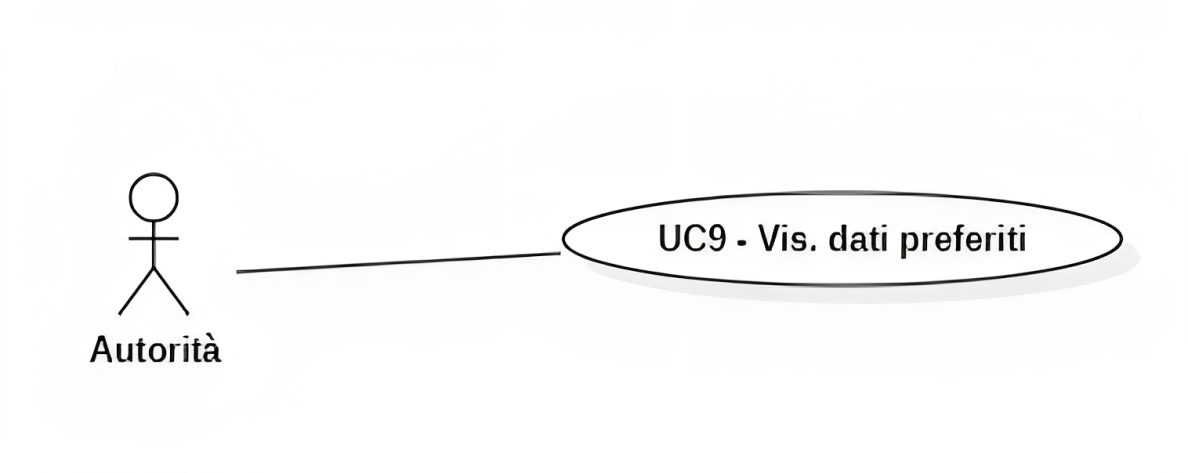
\includegraphics[width=0.9\textwidth]{Images/uc9.png}
    \caption{UC9 - Visualizzazione dati preferiti}
    \label{fig:UC9}
\end{figure}

\subsubsection{UC9 - Visualizzazione dati preferiti}
\begin{itemize}
    \item \textbf{Attore principale:} Autorità locale;
    \item \textbf{Descrizione:} L’autorità locale seleziona la visulizzazione dei dati preferiti.
    \item \textbf{Scenario principale:}
          \begin{enumerate}
              \item L'utente accede alla piattaforma per la visualizzazione della dashboard sullo stato della città o di una cella(UC1) (UC1.1);
              \item L'utente sceglie di visualizzare la pagina dedicata alla visualizzazione dei dati preferiti.
          \end{enumerate}
    \item \textbf{Precondizioni:}
          \begin{itemize}
              \item  L'utente si trova nella pagina per la visualizzazione delle dashboard (UC1) (UC1.1);
          \end{itemize}
    \item \textbf{Postcondizioni:}
          \begin{itemize}
              \item  L'utente ha una visione dei dati dei sensori salvati come preferiti.
          \end{itemize}
    \item \textbf{User story associata:}
          \begin{itemize}
              \item In qualità di Autorità Locale, desidero visualizzare i dati dei sensori precedentemente salvati come preferiti sulla piattaforma, così da poter accedere rapidamente alle informazioni rilevanti.
          \end{itemize}
\end{itemize}

%______________________________________________________________________%

\begin{figure}[H]
    \centering
    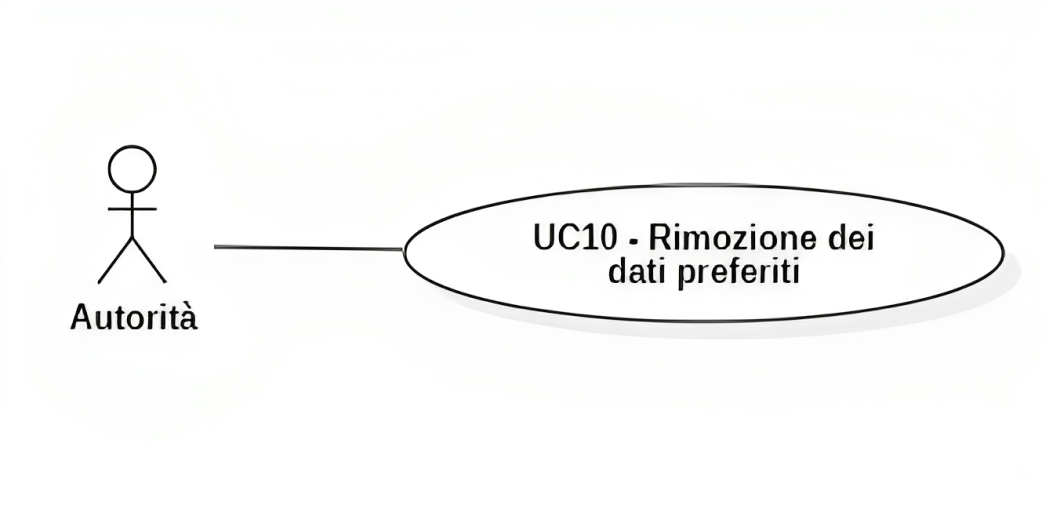
\includegraphics[width=0.9\textwidth]{Images/uc10.png}
    \caption{UC10 - Rimozione dati preferiti}
    \label{fig:UC10}
\end{figure}

\subsubsection{UC10 - Rimozione dati preferiti}
\begin{itemize}
    \item \textbf{Attore principale:} Autorità locale;
    \item \textbf{Descrizione:} L’autorità locale, dalla pagina adibita alla visione dei dati salvati tra i preferiti, rimuove un dato dalla lista.
    \item \textbf{Scenario principale:}
          \begin{enumerate}
              \item L'utente accede alla piattaforma per la visualizzazione della dashboard sullo stato della città o di una cella(UC1) (UC1.1);
              \item L'utente sceglie di visualizzare la pagina dedicata alla visualizzazione dei dati preferiti.
              \item L'utente rimuove uno dei dati dalla lista.
          \end{enumerate}
    \item \textbf{Precondizioni:}
          \begin{itemize}
              \item  L'utente di trova nella pagina per la visulizzazione dei dati preferiti.
          \end{itemize}
    \item \textbf{Postcondizioni:}
          \begin{itemize}
              \item  Il dato del sensore viene rimosso dai preferiti.
          \end{itemize}
    \item \textbf{User story associata:}
          \begin{itemize}
              \item Come autorità locale,
                    Desidero poter rimuovere un dato dalla lista dei preferiti sulla piattaforma,
                    Per poter gestire in modo efficiente i dati visualizzati sulla dashboard.
          \end{itemize}
\end{itemize}

%______________________________________________________________________%
\newcounter{rowcounter}
\setcounter{rowcounter}{1}

\section{Requisiti}
\subsection{Requisiti funzionali}
\begin{longtable}{|C{1cm}|C{2cm}|>{\raggedright}m{5cm}|C{1.5cm}|C{2cm}|}
    \hline
    \textbf{Codice}                                & \textbf{Importanza} & \textbf{Descrizione}                                                                                                                                                                                                               & \textbf{Fonte}  & \textbf{Casi d'uso} \\
    \hline
    RF\arabic{rowcounter}                          & Obbligatorio        & Il prodotto deve essere ad accesso pubblico, ovvero senza login                                                                                                                                                                    & Capitolato      &                     \\
    \hline
    \stepcounter{rowcounter} RF\arabic{rowcounter} & Obbligatorio        & Il prodotto non deve avere una gestione di amministrazione.                                                                                                                                                                        & Capitolato      &                     \\
    \hline
    \stepcounter{rowcounter} RF\arabic{rowcounter} & Obbligatorio        & L'utente deve poter visualizzare una dashboard con una visuale completa sullo stato della città tramite \newline i dati dei sensori, con l'utilizzo di grafici e widget                                                             & Capitolato      & UC1          \\
    \hline
    \stepcounter{rowcounter} RF\arabic{rowcounter} & Obbligatorio        & La dashboard deve essere aggiornata in tempo reale per riflettere immediatamente i dati provenienti dai sensori.                                                                                                                   & Capitolato      & UC1               \\
    \hline
    \stepcounter{rowcounter} RF\arabic{rowcounter} & Obbligatorio        & La piattaforma deve supportare la visualizzazione di dati provenienti da diversi tipi di sensori attivi.                                                                                                                           & Capitolato      & UC1               \\
    \hline
    \stepcounter{rowcounter} RF\arabic{rowcounter} & Obbligatorio        & La dashboard deve presentare grafici interattivi che consentano all'utente di esplorare i dati in dettaglio.                                                                                                                       & Capitolato      & UC1               \\
    \hline
    \stepcounter{rowcounter} RF\arabic{rowcounter} & Obbligatorio        & La dashboard deve presentare un widget separato per ogni tipologia di sensore attivo che trasmette dati al sistema.                                                                                                                & Capitolato      & UC1.1               \\
    \hline
    \stepcounter{rowcounter} RF\arabic{rowcounter} & Obbligatorio        & Ogni widget deve contenere un grafico aggiornato in tempo reale relativo alla tipologia di sensore corrispondente.                                                                                                                 & Capitolato      & UC1.1               \\
    \hline
    \stepcounter{rowcounter} RF\arabic{rowcounter} & Obbligatorio        & La dashboard della città deve includere una mappa interattiva che mostra la posizione dei diversi sensori nella città.                                                                                                             & Capitolato      & UC1.2                   \\
    \hline
    \stepcounter{rowcounter} RF\arabic{rowcounter} & Obbligatorio        & La mappa deve mostrare i sensori posizionati nella città, e ognuno di essi deve essere etichettato in modo da consentire il riconoscimento della tipologia                                                                         & Capitolato      & UC1.2               \\
    \hline
    \stepcounter{rowcounter} RF\arabic{rowcounter} & Obbligatorio        & La dashboard deve fornire un punteggio di salute relativo alla città basato sui dati aggregati provenienti dai sensori.                                                                                                            & Verbale interno & UC1                    \\
    \hline
    %----------------------------------------UC1--------------------------------
    \hline
    \stepcounter{rowcounter} RF\arabic{rowcounter} & Obbligatorio        & L'utente deve avere la possibilità di selezionare una cella, ovvero un'area specifica della città, al fine di visualizzare una dashboard dedicata.& Capitolato      & UC2              \\
    \hline
    \stepcounter{rowcounter} RF\arabic{rowcounter} & Obbligatorio        & Dopo la selezione della cella, il sistema deve mostrare una dashboard contenente esclusivamente i dati correlati a essa.                                                                                                           & Capitolato      & UC2               \\
    \hline
    \stepcounter{rowcounter} RF\arabic{rowcounter} & Obbligatorio        & La dashboard deve essere aggiornata in tempo reale per fornire all'utente una valutazione rapida dello stato complessivo della cella.                                                                                              & Capitolato      & UC2               \\
    \hline
    \stepcounter{rowcounter} RF\arabic{rowcounter} & Obbligatorio        & La dashboard deve presentare grafici interattivi che consentano all'utente di esplorare i dati relativi alla cella in dettaglio.                                                                                                   & Capitolato      & UC2               \\
    \hline
    \stepcounter{rowcounter} RF\arabic{rowcounter} & Obbligatorio        & Il sistema deve presentare un widget per ogni tipologia di sensore attivo nella cella.                                                                                                                                             & Capitolato      & UC2.1               \\
    \hline
    \stepcounter{rowcounter} RF\arabic{rowcounter} & Obbligatorio        & Ogni widget deve contenere un grafico aggiornato in tempo reale relativo alla tipologia di sensore corrispondente presente nella cella.                                                                                            & Capitolato      & UC2.1               \\
    \hline
    \stepcounter{rowcounter} RF\arabic{rowcounter} & Obbligatorio        & L'utente deve poter visualizzare una mappa dei sensori presenti nella cella selezionata.                                                                                                                                           & Capitolato      & UC2.2               \\
    \hline
    \stepcounter{rowcounter} RF\arabic{rowcounter} & Obbligatorio        & La mappa deve mostrare in modo chiaro la posizione di ciascun sensore nella cella.                                                                                                                                                 & Capitolato      & UC2.2               \\
    \hline
    \stepcounter{rowcounter} RF\arabic{rowcounter} & Obbligatorio        & La dashboard deve presentare un punteggio di salute relativo alla cella, basato sull'analisi dei dati provenienti dai sensori.                                                                                                     & Verbale interno      & UC2               \\
    \hline
    \stepcounter{rowcounter} RF\arabic{rowcounter} & Obbligatorio        & L'utente principale (Autorità locale) deve poter selezionare l'opzione per visualizzare i dati storici dei sensori sulla piattaforma.                                                                                              & Capitolato      & UC3               \\
    \hline
    \stepcounter{rowcounter} RF\arabic{rowcounter} & Obbligatorio        & L'utente principale deve essere in grado di selezionare l'arco temporale desiderato per la visualizzazione dei dati storici dei sensori. Di default, la visualizzazione deve includere tutti i dati disponibili.                   & Capitolato      & UC3               \\
    \hline
    \stepcounter{rowcounter} RF\arabic{rowcounter} & Obbligatorio        & L'utente può selezionare l'intervallo temporale desiderato (secondo, minuto, ora, giorno, mese, anno) per aggregare le misurazioni storiche in base al corrispondente (secondo, minuto, ora, giorno, mese, anno) di registrazione. & Capitolato      & UC14               \\
    \hline
    \stepcounter{rowcounter} RF\arabic{rowcounter} & Obbligatorio        &     Il sistema deve adattare dinamicamente la rappresentazione dei dati, inclusi i grafici, secondo l'intervallo temporale di aggregazione selezionato dall'utente. & Capitolato      & UC14               \\
    \hline

    \stepcounter{rowcounter} RF\arabic{rowcounter} & Obbligatorio        & Il sistema deve verificare la validità delle date inserite dall'utente.
                                                   & Capitolato          & UC3                                                                                                                                                                                                                                                                      \\
    \hline
    \stepcounter{rowcounter} RF\arabic{rowcounter} & Obbligatorio        & In caso di date non valide, il sistema deve generare una notifica di errore.
                                                   & Capitolato          & UC8                                                                                                                                                                                                                                                                      \\
    \hline
    \stepcounter{rowcounter} RF\arabic{rowcounter} & Obbligatorio        & La notifica di errore deve richiedere all'utente di reinserire date valide.
                                                   & Capitolato          & UC8                                                                                                                                                                                                                                                                      \\
    \hline
    \stepcounter{rowcounter} RF\arabic{rowcounter} & Obbligatorio        & La notifica di errore deve essere chiara e informativa, indicando il motivo specifico dell'invalidità delle date (data fine precedente a data inizio, arco temporale precedente o antecedente all'inizio della trasmissione dati).
                                                   & Capitolato          & UC8                                                                                                                                                                                                                                                                      \\
    \hline
    \stepcounter{rowcounter} RF\arabic{rowcounter} & Obbligatorio        & Dopo aver ricevuto la notifica di errore, l'utente deve essere in grado di correggere immediatamente le date delimitanti.
                                                   & Capitolato          & UC8                                                                                                                                                                                                                                                                      \\

    \hline
    %__________________________________________________________

    \stepcounter{rowcounter} RF\arabic{rowcounter} & Obbligatorio        & Il sistema deve fornire un'opzione per l'impostazione della visualizzazione dello storico dati in formato testuale.                                                                                                                & Capitolato      & UC4               \\
    \hline
    \stepcounter{rowcounter} RF\arabic{rowcounter} & Obbligatorio        & La visualizzazione testuale dello storico dati deve presentare le informazioni nel formato (TIMESTAMP, Dato).                                                                                                                      & Capitolato      & UC4               \\
    \hline
    \stepcounter{rowcounter} RF\arabic{rowcounter} & Obbligatorio        & L'utente deve poter impostare l'ordine di visualizzazione dei dati in modo crescente rispetto alle misurazioni del sensore.    & Capitolato      & UC11               \\
    \hline
    \stepcounter{rowcounter} RF\arabic{rowcounter} & Obbligatorio        & L'utente deve poter impostare l'ordine di visualizzazione dei dati in modo decrescente rispetto alle misurazioni del sensore.    & Capitolato      & UC12               \\
    \hline
    \stepcounter{rowcounter} RF\arabic{rowcounter} & Obbligatorio        &  Il sistema deve fornire all'utente la possibilità di specificare due valori (minimo e massimo) per il filtraggio della visualizzazione storica delle sole misurazioni del/i sensore/i che hanno il dato acquisito dall'ambiento compreso tra i valori.       & Capitolato      & UC13               \\
    \hline
    \stepcounter{rowcounter} RF\arabic{rowcounter} & Obbligatorio        &  L'utente deve essere in grado di rimuovere il filtro di visualizzazione delle sole misurazioni tra due valori e ripristinare la visualizzazione completa dello storico dei dati.    & Capitolato      & UC13               \\
    \hline
    \stepcounter{rowcounter} RF\arabic{rowcounter} & Obbligatorio        & L'utente deve avere la possibilità di impostare la visualizzazione dei dati storici in formato grafico.                                                                                                                   & Capitolato      & UC5               \\
    \hline
    \stepcounter{rowcounter} RF\arabic{rowcounter} & Obbligatorio        & L'utente deve poter visualizzare lo storico dei dati trasmessi da una specifica categoria di sensori presenti nella città in formato grafico                                                                                       & Capitolato      & UC3.1, UC5               \\
    \hline
    \stepcounter{rowcounter} RF\arabic{rowcounter} & Obbligatorio        & L'utente deve poter visualizzare lo storico dei dati trasmessi da una specifica categoria di sensori presenti nella \newline città in formato testuale (TIMESTAMP : dato)                                                          & Capitolato & UC3.1, UC4                   \\
    \hline
    \stepcounter{rowcounter} RF\arabic{rowcounter} & Obbligatorio        & L'utente deve poter visualizzare lo storico dei dati trasmessi da una specifica categoria di sensori presenti in una cella in formato grafico                                                                                      & Capitolato      & UC3.2, UC5             \\
    \hline
    \stepcounter{rowcounter} RF\arabic{rowcounter} & Obbligatorio        & L'utente deve poter visualizzare lo storico dei dati trasmessi da una specifica categoria di sensori presenti in \newline una cella in formato testuale (TIMESTAMP : dato)                                                         & Capitolato & UC3.2, UC4                \\
    \hline
    \stepcounter{rowcounter} RF\arabic{rowcounter} & Obbligatorio        & L'utente deve poter visualizzare lo storico dei dati trasmessi da un sensore in formato grafico                                                                                                                                    & Capitolato & UC3.3, UC5                 \\
    \hline
    \stepcounter{rowcounter} RF\arabic{rowcounter} & Obbligatorio        & L'utente deve poter visualizzare lo storico dei dati trasmessi da un sensore in formato testuale (TIMESTAMP : dato)                                                                                                                & Capitolato & UC3.3, UC4            \\
    \hline
    \stepcounter{rowcounter} RF\arabic{rowcounter} & Obbligatorio        & L'utente deve poter salvare dati storici trasmessi dal/i sensore/i in una lista di preferiti visibile e comune ad ogni utente                                & Verbale interno & UC7               \\
    \hline
    \stepcounter{rowcounter} RF\arabic{rowcounter} & Obbligatorio        & L'utente deve poter salvare dati trasmessi dai sensori di una tipologia nella città nel formato testuale (TipoSensore, TIMESTAMP, Dato) in una lista di preferiti visibile e comune ad ogni utente                                & Verbale interno & UC7.1               \\
    \hline
    \stepcounter{rowcounter} RF\arabic{rowcounter} & Obbligatorio        & L'utente deve poter salvare dati trasmessi dai  sensori di una tipologia nella cella nel formato testuale (Cella, TipoSensore, TIMESTAMP, Dato) in una lista di preferiti visibile e comune ad ogni utente                         & Verbale interno & UC7.2               \\
    \hline
    \stepcounter{rowcounter} RF\arabic{rowcounter} & Obbligatorio        & L'utente deve poter salvare dei dati trasmessi da un sensore nel formato testuale (IDSensore,Cella, TipoSensore, TIMESTAMP, Dato) in una lista di preferiti visibile e comune ad ogni utente                                       & Verbale interno & UC7.3               \\
    \hline
    \stepcounter{rowcounter} RF\arabic{rowcounter} & Obbligatorio        & Prima di salvare il dato tra i preferiti, il sistema deve verificare che il dato non sia già presente nella lista dei preferiti.                                                                                                   & Verbale interno      & UC7               \\
    \hline
    \stepcounter{rowcounter} RF\arabic{rowcounter} & Obbligatorio        & L'utente deve poter visualizzare la lista dei dati preferiti.                                                                                                                                                                       & Verbale interno & UC9                 \\
    \hline
    \stepcounter{rowcounter} RF\arabic{rowcounter} & Obbligatorio        & L'utente deve poter rimuovere un dato dalla lista dei preferiti.                                                                                                                                                                    & Verbale interno & UC10               \\
    \hline
    \stepcounter{rowcounter} RF\arabic{rowcounter} & Obbligatorio        & L'utente deve essere in grado di visualizzare le informazioni dei sensori.                                                                                                                                                           & Capitolato      & UC6               \\
    \hline
    \stepcounter{rowcounter} RF\arabic{rowcounter} & Obbligatorio        & L'utente deve essere in grado di visualizzare l'ID dei sensori.                                                                                                                                                                    & Capitolato      & UC6.1               \\
    \hline
    \stepcounter{rowcounter} RF\arabic{rowcounter} & Obbligatorio        & L'utente deve essere in grado di visualizzare il tipo dei sensori.                                                                                                                                                                 & Capitolato      & UC6.2               \\
    \hline
    \stepcounter{rowcounter} RF\arabic{rowcounter} & Obbligatorio        & L'utente deve essere in grado di visualizzare la posizione dei sensori in coordinate.                                                                                                                                                            & Capitolato      & UC6.3               \\
    \hline
    \stepcounter{rowcounter} RF\arabic{rowcounter} & Obbligatorio        & L'utente deve essere in grado di visualizzare la cella in cui è installato il sensore.                                                                                                                                                & Capitolato      & UC6.4               \\
    \hline
    \stepcounter{rowcounter} RF\arabic{rowcounter} & Obbligatorio        & L'utente deve essere in grado di visualizzare la data di installazione dei sensori.                                                                                                                                                & Capitolato      & UC6.5               \\
    \hline
    \stepcounter{rowcounter} RF\arabic{rowcounter} & Obbligatorio        & L'utente deve essere in grado di visualizzare l'unità di misura associata al sensore.                                                                                                                                              & Capitolato      & UC6.6               \\
    \hline
\end{longtable}
\subsection{Requisiti qualitativi}
\subsection{Requisiti di vincolo}
\subsection{Tracciamento}

\end{document}